% Modified by Alessio Guglielmi, 3 February 2021

\documentclass[12pt,a4paper]{report}
% This document template assumes you will use pdflatex.  If you are using
% latex and dvipdfmx to translate to pdf, insert dvipdfmx into the options.

\usepackage{Bath-CS-Dissertation}
\usepackage{lmodern}
\usepackage{float}
\usepackage{amsthm}
\usepackage{amssymb}
\usepackage{amsmath}
\usepackage{algorithm}
\usepackage{algpseudocode}

\theoremstyle{definition}
\newtheorem{definition}{Definition}[section]

\algblock{Input}{EndInput}


\title{\bf Applying Gaussian Processes in the Sport of Cricket}
\author{Louie Middle}
\date{Bachelor of Science in Computer Science\\ 
                                 % E.g.: Bachelor of Science in Computer Science
                                 %       Master of Science in Data Science
      The University of Bath\\
      2023}

%%%%%%%%%%%%%%%%%%%%%%%%%%%%%%%%%%%%%%%%%%%%%%%%%%%%%%%%%%%%%%%%%%%%%%%%%%%%%%%%
%%%%%%%%%%%%%%%%%%%%%%%%%%%%%%%%%%%%%%%%%%%%%%%%%%%%%%%%%%%%%%%%%%%%%%%%%%%%%%%%
%%%%%%%%%%%%%%%%%%%%%%%%%%%%%%%%%%%%%%%%%%%%%%%%%%%%%%%%%%%%%%%%%%%%%%%%%%%%%%%%
\begin{document}

\hypersetup{pageanchor=false}	

% Set this to the language you want to use in your code listings (if any)
\lstset{language=Java,breaklines,breakatwhitespace,basicstyle=\small}

\setcounter{page}{0}
\pagenumbering{roman}

\maketitle
\newpage

% Set this to the number of years consultation prohibition, or 0 if no limit
\consultation{0}
\newpage

\declaration{Applying Gaussian Processes in the Sport of Cricket}{Louie Middle}
\newpage

\hypersetup{pageanchor=true}

\abstract
$\langle$
The abstract should appear here. 
An abstract is a short paragraph describing the aims of the project, what was achieved and what contributions it has made.
$\rangle$
\newpage

\tableofcontents
\newpage

\listoffigures
\newpage

\listoftables
\newpage

\listofalgorithms
\newpage

%%%%%%%%%%%%%%%%%%%%%%%%%%%%%%%%%%%%%%%%%%%%%%%%%%%%%%%%%%%%%%%%%%%%%%%%%%%%%%%%
%%%%%%%%%%%%%%%%%%%%%%%%%%%%%%%%%%%%%%%%%%%%%%%%%%%%%%%%%%%%%%%%%%%%%%%%%%%%%%%%
\addcontentsline{toc}{chapter}{Acknowledgements}
\chapter*{Acknowledgements}

I would like to acknowledge my supervisor Adam Hartshorne.
I would like to acknowledge my partner Hoi Ching Leung.
I would like to acknowledge my parents.

\newpage
\setcounter{page}{1}
\pagenumbering{arabic}

%%%%%%%%%%%%%%%%%%%%%%%%%%%%%%%%%%%%%%%%%%%%%%%%%%%%%%%%%%%%%%%%%%%%%%%%%%%%%%%%
%%%%%%%%%%%%%%%%%%%%%%%%%%%%%%%%%%%%%%%%%%%%%%%%%%%%%%%%%%%%%%%%%%%%%%%%%%%%%%%%
\chapter{Introduction}

Over the last few decades the amount of data driven techniques to improve the outcomes of sports games has increased greatly. 
The multi-billion pound market of cricket is no exception. 
There is a strong incentive to improve the techniques used to better the results of teams. 
This study aims to investigate the possibility of predicting the outcome of a bowler batter match-up in cricket using modern machine learning techniques and how this could then aid cricket bowling choices and team selection. 
The main training and testing data will be the 2022 Indian Premier League (IPL) season (TODO: Change)
The hope is that using knowledge of bowler pitch trajectories and batter shot trajectories gathered from modern ball tracking will add another layer of granularity in addition to simply considering the resultant runs scored of each delivery. 
Furthermore, building a model which can incorporate pitch, atmospheric and ground conditions could further improve any models. 

\section{Moneyball}

The release of Moneyball \citep{Moneyball2004}, was a big driver in the increased use of statistical driven techniques in Baseball player selection and scouting techniques. 
Pioneered by the likes of Bill James and Sabermetrics, Moneyball has entered baseball's lexicon; teams that value Sabermetrics are often said to be playing "Moneyball".  
One of the notable benefits of a Moneyball approach is in reducing player salaries, whilst maintaining high performance. 
Notable recent Moneyball successes include the Tampa Bays, whose entire 2019 roster was around 63\% of the total budget of the \$40 million the Houston Astros were spending on Gerrit Cole's contract. 
It was reported that the Rays spending totalled \$648,000 per victory, compared to the Astros \$1.54 million per win.
Despite this large difference pay, the Rays still had a successful season and finished second in the American League East \citep{Fox2019}.

Similar successes can be found in other sports, such as association football (or soccer). 
In 2010 Liverpool F.C. were purchased by Boston Red Sox owner John W. Henry. 
With the Red Sox, Henry hired Sabermetrics pioneer Bill James and their Moneyball approach saw the team win the World Series in 2004, 2007, 2013 and 2018. 
With Liverpool, Henry hired University of Cambridge PhD Ian Graham in 2012 as head of analysis and J\"urgen Klopp as Manager in 2015 \citep{Liverpool2022}. 
Graham influenced the signings of key players, such as Mohammed Salah, Philippe Coutinho and Naby Ke\"ita. 
Grahams data suggested Salah would pair especially well with Roberto Firmino, who creates more expected goals than nearly anyone else in his position \citep{Liverpool2019}. 
Expected goals turned to real goals in the 2017-2018 season, with Salah scoring 32 goals and Firmino scoring 15. 
The combination of Klopp and his intuitive knowledge, mixed with the likes of Grahams data-driven knowledge, has led to Liverpool having fantastic recent success winning the 2018-2019 UEFA Champions League and the 2019-2020 English Premier League.

\section{Indian Premier League}

The Indian Premier League (IPL) is a professional cricket league based on the Twenty20 format. 
As reported by \citet{ESPNcricinfo2018}, Star Sports invested \$2.55 billion for exclusive broadcasting rights for the 2018 IPL season. 
This season saw a 29\% increment in the number of viewers, through both digital streaming and television. 
The interest in the IPL is clear to see, thus increasing the desire to use modern techniques to improve results.

\section{Project Plan}

TODO: This can be removed

There are 26 weeks from Friday the 4th November until the final deadline of Friday the 5th May. 
The individual project is 24 credits out of a total 60 credits for the year, meaning 40\% of my time can be used for the project. 
This is 10.4 weeks. 
To allow for buffer and holidays I will assume I have 8 working weeks to complete the project. 
I have split my project into 3 main sections:

\begin{enumerate}
    \item Literature review and pre-processing (2 weeks)
    \item Developing and improving models (4 weeks)
    \item Analysis of models and write up (2 weeks)
\end{enumerate}

The buffer time can be used for any road bumps, or sections that need it. 
See Gantt chart for overview of plan in figure \ref{fig:gantt_chart}.

\begin{figure}[H]
    \centering
    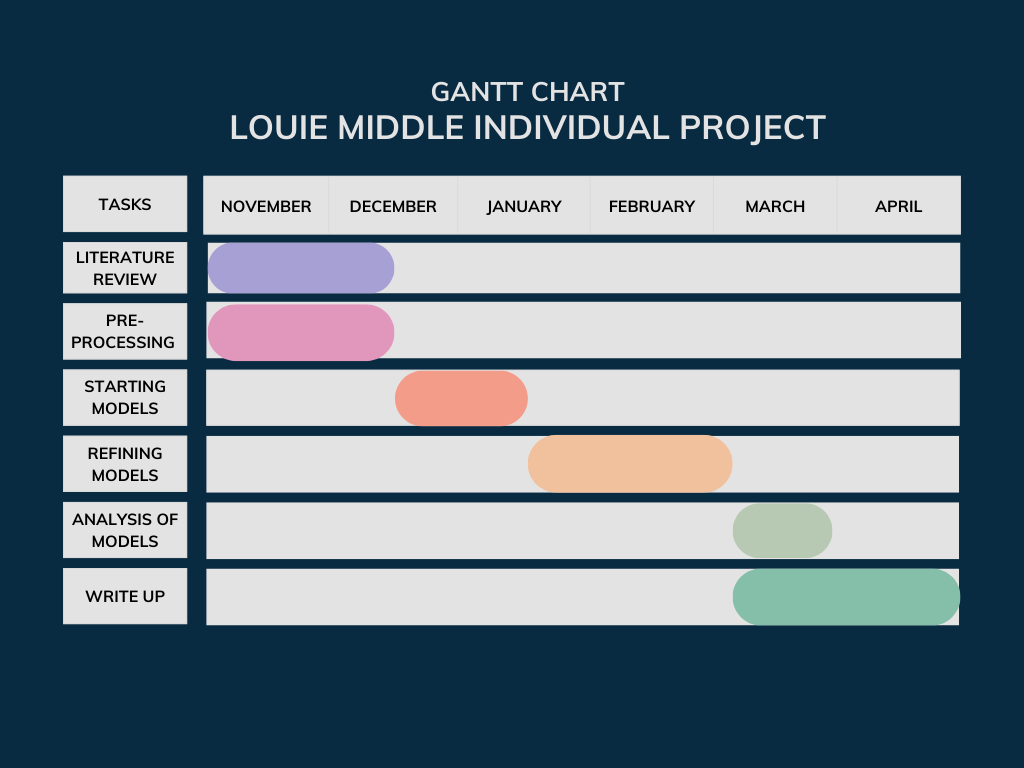
\includegraphics[width=\linewidth]{Gantt Chart.png}
    \caption{Gantt Chart For Project}
    \label{fig:gantt_chart}
\end{figure}

\section{Resources Required}

TODO: This section should be removed or amended. I think get some data from just one year, or all years and compare to test Horvat and Job.

In order to train any machine learning model an appropriate amount of data for training and testing. 
Because it is not beneficial to use data that is too old \citep{horvat2020}, a recent season's worth of data would be good, saving some data for testing. 

Training machine learning models may also require appropriate computing power depending on the models used and size of the data set. 
This could potentially be achieved with the University of Bath's Hex cluster.

%%%%%%%%%%%%%%%%%%%%%%%%%%%%%%%%%%%%%%%%%%%%%%%%%%%%%%%%%%%%%%%%%%%%%%%%%%%%%%%%
%%%%%%%%%%%%%%%%%%%%%%%%%%%%%%%%%%%%%%%%%%%%%%%%%%%%%%%%%%%%%%%%%%%%%%%%%%%%%%%%
\chapter{Literature and Technology Survey}

\section{Existing Machine Learning in Sport}

\begin{figure}[H]
    \centering
    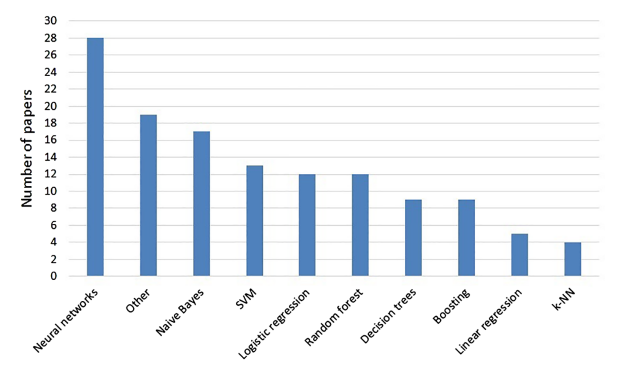
\includegraphics[width=\linewidth]{Horvat&Job_Figure2.png}
    \caption{Number of papers using a particular ML algorithm group \citep{horvat2020}}
    \label{fig:NoPapers}
\end{figure}

TODO: Could be worth putting the one with publication year in to show uptick in research? But not necessary right now.

Figure \ref{fig:NoPapers} from \citet{horvat2020}'s literature review of machine learning in sport for score prediction shows what current methods are currently used in the field as of May 2020. 
As you can see, neural networks have a large research output, followed by other popular methods such as regression, SVMs, regression, decision trees, and gradient boosting with k-NN being the least used. 
It is important to note, that just because a large body of research has been carried out with certain methods, it does not necessarily mean they are the best. 

\citet{horvat2020} also showed that including too many seasons worth of data for training models reduces the quality of results. 
To those with a basic knowledge of cricket and sport this is not surprising given that in just a few years, many things related to team composition and tactics can change. 
The best prediction results were achieved by researchers who used data from a single season and a data segmentation evaluation method. 
When using data from a single season, most of the data is used for training and a small portion for testing. 
Some researchers used the same data set for training and testing yielding unrealistically accurate results.

\section{Existing Machine Learning in Cricket}

\citet{KampakisStylianos2015} used Naïve Bayes, logistic regression, random forests and gradient boosted decision trees to predict the outcome of English County 20 over Cricket Matches from 2009 - 2014. 
The performance of each algorithm was assessed using one year's data as the training data set and the following year's data for testing. 
Each model was tested over these seasons and achieved an accuracy of 62.4\% for Naïve Bayes, 60.1\% for logistic regression, 55.6\% for random forests and 57.2\% for decision trees.

\subsection{Existing Machine Learning in the Indian Premier League}

\citet{Saikia2012} have used Artificial Neural Network models to predict the performance of bowlers based on their performance in the first three seasons of the IPL. 
When the predicted results were validated with the players performances in the fourth season, the model had an accuracy of 71.43\%.

\section{Research with similar goals}

The Singlearity-PA model \citep{silver2021baseball} wanted to attempt to solve one of the most fundamental questions in baseball:	 How can we	predict the outcome of a batter	vs. pitcher plate appearance (PA)? 
This is similar to my goal with cricket:  To predict the outcome of batter vs bowler for an over.

The Singlearity-PA model \citep{silver2021baseball} was able to accurately predict the results of a batter versus pitcher plate appearance using a neural-network based AI model. 
The details of the model used are vague, however the network was able to take in 87 inputs and then output probabilities for each of the 21 possible outcomes of a plate appearance (PA) in baseball. 
Comparisons can be made between this and cricket. 
A plate appearance can be compared to an over, comprising 6 balls (or more including no balls and wides) between a single bowler and 1 or more batsmen. 
The outcome of the over could be considered to be the runs scored. 

\citet{silver2021baseball} also split their player base up by how many PAs they had for each player. 
The best players had greater than 500 PAs worth of data each, but the vast majority had less than 100. 
SinglearityPA was able to accurately predict the result of match-ups for these players with fewer PAs better than existing solutions. 
Parallels can be drawn between this and cricket, as there are often players who have little data, yet team selectors would want to know who the best player is to match-up against them.

Extending Singlearity-PA with Markov chains improved more complicated strategies, such as optimal player lineups or to decide on pinch hitters and relief pitchers. 
Similarly, in cricket the batting lineup and choice of bowler at different points in a game have a large impact on the score. 
In the example provided, Singlearity-PA's predicted runs scored for an optimal lineup was 6.7\% better than the actual lineup in the 2019 National League All-Star game. 
It is important not to compare baseball and cricket too closely, but the techniques used by Silver and Huffman could potentially work well in Cricket.

\section{Drawbacks of Existing Methods}

Sport outcome predictors are most commonly used by supervised ML methods, typically classification methods or regression methods \citep{horvat2020}. 
Whilst existing research can achieve impressive results, surprises in sport still happen. For example, the odds of Leicester City winning the Premier League in the 2015/2016 season were 1-5000. 
However, analysis of their performances show their title was absolutely deserved.

This could be explained in that a problem with existing models is that they only output a single value. 
There is no uncertainty in the output as to how confident the model is in its prediction. 
This has a problem in that making decisions based on this prediction becomes much more difficult, as decision makers can't be sure how much to trust the prediction. 
Furthermore, certain inputs exist where very little similar training data might exist. 
In such cases, the uncertainty in a models output should be much greater. 
Yet, existing models will still provide a prediction the same as it would for inputs where there was a large amount of training data.

 TODO: talk about \citep{Blumberg2020}.

\section{Gaussian Processes in Sport}

TODO: Talk about Gaussian processes in sport

\chapter{Background}

In this chapter I will cover the requisite background for Gaussian processes and gradient boosting, the two key methods used in this project.

\section{Gaussian Processes}

\citep{Griffiths2023}

\citep{RasmussenWilliams2006}

\citep{Kaiser2017}

\citep{Yi2019} TODO: This has good explanations of stuff

TODO: Put cholesky decomposition and KL divergence in the appendix

This section introduces Gaussian processes and the following section then explains how to extend their application to solve data association problems. 
This project is mostly concerned with using Gaussian processes for classification, but a background on using Gaussian processes for regression is provided first as a basis before their extension to classification tasks. 
As Gaussian processes are not computationally cheap sparse approximations were used in this project and are also reviewed in this section.

Gaussian processes are a non-parametric regression model. 
\emph{Non-parametric models} are not based on insights about the concrete structure of the function to be modelled, but instead make assumptions about the function itself, such as its smoothness or differentiability. 
Instead of modeling a distribution of parameter values, a non-parametric model tries to find a distribution $p(f*)$ of probable functions that represents the function $f$ to be estimated.

In addition, Gaussian processes are a supervised learning technique, where we start with a training data set $\mathcal{D}$ of $n$ observations, $\mathcal{D} = (\textbf{x}_{i}, y_{i} | i = 1, ..., n)$ where $\textbf{x}$ denotes an input vector (covariates) of dimension $D$ and $y$ denotes an output or target. 
The column vector inputs for all $n$ cases are aggregated in the $D x n$ design matrix $X$ and the targets collected in the vector $\textbf{y}$, such that $\mathcal{D} = (X, \textbf{y})$.

\subsection{Gaussian Processes for Regression}

\subsubsection{Weight Space View}

TODO: This section might not be necessary, but might be good to show understanding....

One can think of a Gaussian process as defining a distribution over functions and inference taking place directly in the space of functions. 
Although this view is appealing, it is difficult to grasp on first attempt, and so we will start with reviewing the \emph{weight-space view}.

First, lets review the standard linear regression model with Gaussian noise

\begin{equation}
    \centering
    {f(\textbf{x}) = \textbf{x}^T\textbf{w}, \quad y = f(\textbf{x}) + \epsilon}
\end{equation}

where $\textbf{x}$ is the input vector, $\textbf{w}$ is a vector of weights of the linear model, $f$ is the function value, and $y$ is the observed target value.
It is often assumed that the observed values differ from the function values by some noise, which we will treat as an independent, identically distributed Gaussian distribution, with zero mean and variance $\sigma^2_{n}$.

\begin{equation}
    \centering
    \epsilon \sim \mathcal{N}(0, \sigma^2_{n})
\end{equation}

This noise assumption together with the model gives rise to the likelihood, the probability density of the observations given the parameters, which is factored over cases in the training set to give

\begin{equation}
    \centering
    p(\textbf{y} | X, \textbf{w}) = \prod_{i=1}^n = p(y_{i} | \textbf{x}_{i}, \textbf{w}) =  \prod_{i=1}^n \frac{1}{\sqrt{2\pi}\sigma_{n}} exp(-\frac{(y_{i} - \textbf{x}_{i}^T \textbf{w})^2}{2 \sigma_{n}^2})
    TODO: Can do the rest later
\end{equation}

We put a zero mean Gaussian prior with covariance matrix $\Sigma_{p}$ on the weights 

\begin{equation}
    \centering
    \textbf{w} \sim \mathcal{N}(0, \Sigma_{p})
\end{equation}

Inference is based on the posterior distribution over the weights computed by Baye's rule, given by

\begin{equation}
	\centering
	P(\textbf{w} | \textbf{y}, X)  = \frac{p(\textbf{y} | X, \textbf{w})p(\textbf{w})}{p(\textbf{y} | X)}
\end{equation}

Note that prior $p(\textbf{w})$ neglects the conditioning on $X$, as it is independent of the inputs. The normalising constant $p(\textbf{y} | X)$, also know as the marginal likelihood is independent of the weights and is given by

\begin{equation}
	\centering
	P(\textbf{y} | X)  = \int p(\textbf{y} | X, \textbf{w})p(\textbf{w}) d\textbf{w}
\end{equation}

Since the number of obervations is finite and the function $f$ lives in an infinite dimensional function space, the estimation of $f$ is uncertain and based on prior assumptions about its structure.

TODO: Finish this later when you can ask Adam about it....

To make predictions we average over all possible parameter values, weighted by their posterior probability.
Thus the predictive distribution for $f_{*} \triangleq f(\textbf{x}_{*})$ at $\textbf{x}_{*}$ is given by averaging the output of all possible linear models w.r.t the Gaussian posterior

\begin{equation}
	\begin{aligned}
		\centering 
		p(f_{*} | \textbf{x}_{*}, X, \textbf{y}) &= \int p(f_{*} | \textbf{x}_{*}, \textbf{w})p(\textbf{w} | X, \textbf{y}) d\textbf{w}\\
		&= \mathcal{N}(\frac{1}{\sigma_{n}^2} \textbf{x}_{*}^T A^{-1} X \textbf{y}, \enskip \textbf{x}_{*}^T A^{-1} \textbf{x}_{*}).
	\end{aligned}
\end{equation}

The predictive distribution is again Gaussian.

\subsubsection{Function-space View}

\begin{definition}[Gaussian Process]
A Gaussian process is a collection of random variables, any finite number of which have a joint Gaussian distribution. 
\end{definition}

Gaussian processes are a generalisation of the Gaussian distribution to function spaces. 
A multivariate Gaussian $\textbf{x} \sim \mathcal{N} (\boldsymbol{\mu}, \boldsymbol{\Sigma})$ describes a distribution over the finitely many elements in the vector $\textbf{x}$. 
Every element of $\textbf{x}$ is normally distributed. 
For two points in $\textbf{x}$, $x_{i}$ and $x_{j}$, their covariance is given by $cov[x_{i}, x_{j}] = \Sigma_{ij}$.

A Gaussian process is completely specified by its mean function, $m(\textbf{x})$, and its co-variance function $k(\textbf{x}, \textbf{x}')$.
Usually the mean function is assumed to be constant zero, but this need not be the case.
A mean function and covariance function can be defined for a real process $f(x)$ as 

\begin{equation}
	\begin{aligned}
		\centering
		m(\textbf{x}) &= \mathbb{E}[f(\textbf{x})],\\
		k(\textbf{x}, \textbf{x}') &= \mathbb{E}[(f(\textbf{x}) - m(\textbf{x}))(f(\textbf{x}') - m(\textbf{x}'))],
	\end{aligned}
\end{equation}

where we will write the Gaussian process as 

\begin{equation}
	\centering
	f(\textbf{x}) \sim GP(m(\textbf{x}), k(\textbf{x}, \textbf{x}')).
\end{equation}

The covariance function, also called a kernel, specifies the covariance between pairs of random variables. It is the covariance functions which encode the assumptions about the underlying function (see section \ref{sec:Kernels}).

\subsection{Kernels} \label{sec:Kernels}

Kernels are crucial in encoding the assumptions about the function a Gaussian process should estimate. 
It is a measure of similarity of different points in the observed data and of new points to be predicted. 
For example, a natural assumption is to assume the closer two points lie, the more similar their function values should be. 
Furthermore, when prediciting test points, training points close to it are probably more informative than those further away. 
However, it should be noted, that this need not be the case. 
For example, consider a sinusoidal wave where two points which are multiple wavelengths apart should have similar function values.
A kernel that only depends on the distance between two points is called \emph{stationary}.
Conversely, kernels that do depend on two points position in the input space are called \emph{non-stationary}.

A common kernel and one used throughout this project is the squared exponential (SE) covariance function (also known as the radial basis function, RBF). 
This is defined by

\begin{equation}
	\centering
	cov(f(\textbf{x}), f(\textbf{x}')) = k(\textbf{x}, \textbf{x}') = exp(-\frac{1}{2} |\textbf{x}_{p} - \textbf{x}_{q}|^2).
	\label{eq:SquaredExponentialKernel}
\end{equation}

Kernels have characteristic length scales which informally can be thought of as roughly the distance you have to move in input space before the function value will change significantly. 
For eq \ref{eq:SquaredExponentialKernel} the length-scale is one. 
By replacing $\textbf{x}_{p} - \textbf{x}_{q}$ with $\textbf{x}_{p} - \textbf{x}_{q} / l$ for some positive constant $l$ we can change the characteristic length-scale of the process.
Choice of such parameters will be discussed more later.

TODO: Explain $\sigma$ !!!

\begin{figure}[H]
   	 \begin{minipage}[t]{0.3\textwidth}
	 	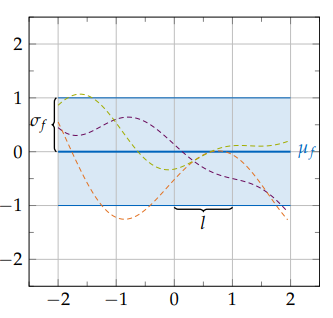
\includegraphics[width=\linewidth]{RBF_sigma_1_lengthscale_1.png}
	    	\caption{SE kernel with $\sigma=1$ and $l=1$ \citep{Kaiser2017}}
	    	\label{fig:SEKernSig1Length1}
	\end{minipage}
	\hfill
	\begin{minipage}[t]{0.3\textwidth}
	 	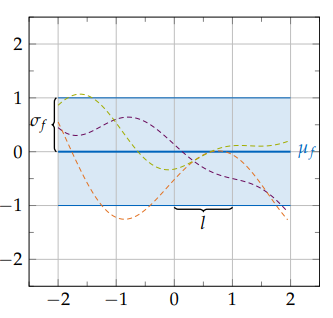
\includegraphics[width=\linewidth]{RBF_sigma_1_lengthscale_1.png}
	    	\caption{SE kernel with $\sigma=\sqrt{2}$ and $l=1$ \citep{Kaiser2017}}
	    	\label{fig:SEKernSigRoot2Length1}
	\end{minipage}
	\hfill
	\begin{minipage}[t]{0.3\textwidth}
	 	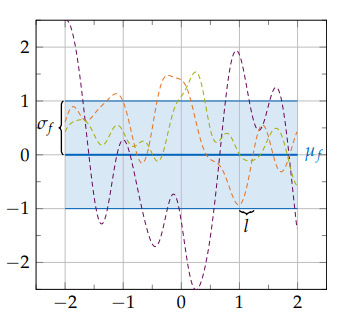
\includegraphics[width=\linewidth]{RBF_sigma_1_lengthscale_025.png}
	    	\caption{SE kernel with $\sigma=1$ and $l=0.25$ \citep{Kaiser2017}}
	    	\label{fig:SEKernSig1Length0.25}
	\end{minipage}
\end{figure}

Figure \ref{fig:SEKernSig1Length1}, figure \ref{fig:SEKernSigRoot2Length1} and figure \ref{fig:SEKernSig1Length0.25} compare sample functions drawn from Gaussian processes with SE kernels with different hyperparameters. 
Since the mean function $m(x)$ is assumed to be constant zero, the kernel specifies the prior assumptions about the function.
The SE kernel describes arbritrary smooth functions. The hyperparameters $l$ and $\sigma$ of the kernel describe the dynamic range in the $x$ and $y$ directions respectively.

\subsection{Predictions and Posterior}

In order to use Gaussian processes for regression, it is necessary to combine observations with a Gaussian process prior $f \sim GP(0, K)$. 
The distribution is obtained by integrating over all possible latent function values $f$ and therefore taking all possible functions into account. This is called the \emph{marginilisation of $f$}. 

The joint distribution of the training outputs, $\textbf{y}$, and the test outputs $\textbf{f}_{*}$ according to the prior is 

\begin{equation}
	\centering
	\begin{bmatrix}
		\textbf{y} \\
		\textbf{f}_{*}
	\end{bmatrix}
	\sim \mathcal{N} \left( 0,
	\begin{bmatrix}
		K(X, X) + \sigma_{n}^2I & K(X, X_{*}) \\
		K(X_{*},  X) & K(X_{*},  X_{*})
	\end{bmatrix} \right) .
	\label{eq:JointPriorDist}
\end{equation}

If there are $n$ training points and $n_{*}$ test points then $K(X, X_{*})$ denotes the $n x n_{*}$ matrix of covariances evaluated at all pairs of training and test points, and similarly for $K(X, X)$, $K(X_{*},  X)$ and $K(X_{*},  X_{*})$.

Using this we arrive at the key predicitve equations for Gaussian process regression

\begin{equation}
	\textbf{f}_{*} | X, \textbf{y}, X_{*} \sim \mathcal{N}(\overline{\textbf{f}}_{*}, cov(\textbf{f}_{*}))
\end{equation}
\begin{equation}
	\overline{\textbf{f}}_{*} \triangleq \mathbb{E}[\textbf{f}_{*} | X, \textbf{y}, X_{*}] = K(X, X_{*})[K(X, X) +  \sigma_{n}^2I]^-1 \textbf{y}
	\label{eq:MeanFunc}
\end{equation}
\begin{equation}
	cov(\textbf{f}_{*}) = K(X_{*}, X_{*}) - K(X_{*}, X)[K(X, X) +  \sigma_{n}^2I]^-1 K(X, X_{*})
	\label{eq:CovarianceFunc}
\end{equation}

Eq. \ref{eq:MeanFunc} and eq. \ref{eq:CovarianceFunc} represent the mean function and the covariance function of the Gaussian posterior process respectively. 

From here forwards, a compact form of $K(X, X)$ and $K(X_{*}, X_{*})$ etc. will be introduced where $K = K(X, X)$ and $K_{*} = K(X, X_{*})$.

Computing $[K + \sigma_{n}^2I]^-1$ costs $O(N^3)$, but can be done as a preprocessing step since it is independent of the test points. 
After this, each single test point costs $O(N)$. 
To predict its variance it is still necessary to perform matrix multiplication which costs $O(N^2)$.

\subsubsection{Marginal Likelihood}

The \emph{marginal likelihood} is the marginalisation over the function values $\textbf{f}$. 
By observing that $\textbf{y} \sim \mathcal{N} (0, K + \sigma_{n}^2I)$ yields the log marginal likelihood

\begin{equation}
	\label{eq:LogMargLik}
	\centering
	\log p(\textbf{y} | X) = -\frac{1}{2}\textbf{y}^T(K +  \sigma_{n}^2I)^-1\textbf{y} - -\frac{1}{2}log|K +  \sigma_{n}^2I| - \frac{n}{2}log2\pi.
\end{equation}

With this, we can create an algorithm for Gaussian process regression, which is given in alg. \ref{alg:GPR}. The matrix inversion required by eq. \ref{eq:MeanFunc} and \ref{eq:CovarianceFunc} uses Cholesky factorisation, explained in section \ref{sec:CholFac}. 

\begin{algorithm}
	\caption{Algorithm for Gaussian process regression}
	\label{alg:GPR}
	\begin{algorithmic}[1]
		\Require $X$ (inputs), \textbf{y} (targets), $k$ (covariance function), $\sigma_{n}^2$ (noise level), $X_{*}$ (test input)	
		\State $L \gets cholesky(K +\sigma_{n}^2I)$
		\State $\boldsymbol{\alpha} \gets L^T \setminus (L \setminus \textbf{y})$ \Comment{eq. \ref{eq:MeanFunc}}
		\State $\overline{f}_{*} \gets \textbf{k}_{*}^T \boldsymbol{\alpha}$ \Comment{eq. \ref{eq:MeanFunc}}
		\State $\textbf{v} \gets L \setminus \textbf{k}_{*}$ \Comment{eq. \ref{eq:CovarianceFunc}}
		\State $\mathbb{V}[f_{*}] \gets k(X_{*}, X_{*}) - \textbf{v}^T\textbf{v}$ \Comment{eq. \ref{eq:CovarianceFunc}}
		\State $\log p(\textbf{y} | X) \gets -\frac{1}{2} \textbf{y}^T \boldsymbol{\alpha} - \Sigma_{i} \log L_{ii} - \frac{n}{2} \log2\pi$ \Comment{eq. \ref{eq:LogMargLik}}
		\State \textbf{return}: $\overline{f}_{*}$ (mean), $\mathbb{V}[f_{*}]$ (variance), $\log p(\textbf{y} | X)$ (log marginal likelihood)
	\end{algorithmic}
\end{algorithm}

\subsubsection{Loss Function}

For practical applications, we are forced to make a decision how to act - we need a point prediction. 
To achieve this, we need a \emph{loss function} $\mathcal{L}(y_{true}, y_{guess})$ which specifies the loss incurred by guessing the value $y_{guess}$ when the true value is $y_{true}$. 

TODO: Loss functions...

\subsection{Gaussian Processes for Classification}

A Gaussian process is a generalisation of the gaussian probability distribution. 
Both classification and regression can be seen as function approximation problems. 
Unfortunately, the solution of classification problems using Gaussian processes is tougher than regression problems. 
For regression problems, the likelihood is often assumed to be Gaussian. 
A Gaussian process prior combined with a Gaussian likelihood gives a posterior Gaussian process over functions, where everything remains analytically tractable. 
For classification models, the Gaussian likelihood is inappropriate; a different likelihood such as a Bernoulli likelihood must be used.

\subsection{Sparse Gaussian Processes}

TODO: Write about sparse GPs

\section{Data Association with Gaussian Processes}

\subsection{Data Association}

\begin{figure}[H]
    \centering
    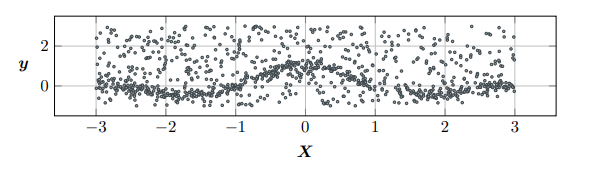
\includegraphics[width=\linewidth]{data_association_problem.png}
    \caption{A data association problem consisting of two generating processes, one of which is a signl we wish to recover and one is an uncorrelated noise process \citep{Kaiser2018}}
    \label{fig:DataAssocProblem}
\end{figure}

A \emph{data association problem} is one where we consider the data to have been generated by a mixture of processes and we are interested in factorising the data into these components. For example, as described by \citet{Kaiser2018}, figure \ref{fig:DataAssocProblem} could represent faulty sensor data, where sensor readings are disturbed by uncorrelated and asymettric noise. Standard machine learning approaches can pollute any models, where the model starts to explain the noise instead of the underlying signal. 

The cricket dataset could be deemed a data association problem....

\citep{Kaiser2018}
\citep{Lui2020}

\section{Gradient Boosting}

TODO: Describe XGBoost

%% NOTE Replace the following with chapters that are appropriate for your
%%      style of project.  It is unlikely these will fit your project perfectly.

%%%%%%%%%%%%%%%%%%%%%%%%%%%%%%%%%%%%%%%%%%%%%%%%%%%%%%%%%%%%%%%%%%%%%%%%%%%%%%%%
%%%%%%%%%%%%%%%%%%%%%%%%%%%%%%%%%%%%%%%%%%%%%%%%%%%%%%%%%%%%%%%%%%%%%%%%%%%%%%%%
\chapter{Method}

%%%%%%%%%%%%%%%%%%%%%%%%%%%%%%%%%%%%%%%%%%%%%%%%%%%%%%%%%%%%%%%%%%%%%%%%%%%%%%%%
%%%%%%%%%%%%%%%%%%%%%%%%%%%%%%%%%%%%%%%%%%%%%%%%%%%%%%%%%%%%%%%%%%%%%%%%%%%%%%%%
\chapter{Results}

%%%%%%%%%%%%%%%%%%%%%%%%%%%%%%%%%%%%%%%%%%%%%%%%%%%%%%%%%%%%%%%%%%%%%%%%%%%%%%%%
%%%%%%%%%%%%%%%%%%%%%%%%%%%%%%%%%%%%%%%%%%%%%%%%%%%%%%%%%%%%%%%%%%%%%%%%%%%%%%%%
\chapter{Discussion}

%%%%%%%%%%%%%%%%%%%%%%%%%%%%%%%%%%%%%%%%%%%%%%%%%%%%%%%%%%%%%%%%%%%%%%%%%%%%%%%%
%%%%%%%%%%%%%%%%%%%%%%%%%%%%%%%%%%%%%%%%%%%%%%%%%%%%%%%%%%%%%%%%%%%%%%%%%%%%%%%%
\chapter{Conclusion}

Code can be output inline using \verb@\lstinline|some code|@.  For example, this code is inline: \lstinline|public static int example = 0;| (we have used the character \verb@|@ as a delimiter, but any non-reserved character not in the code text can be used.)

Code snippets can be output using the \verb|\begin{lstlisting} ... \end{lstlisting}|
environment with the code given in the environment. For example, consider listing \ref{Example-Code}, below.

\begin{lstlisting}[breaklines,breakatwhitespace,caption={Example code},label=Example-Code]
public static void main() {

  System.out.println("Hello World");

}
\end{lstlisting}

Code listings are produced using the package `listings'.  This has many useful options, so have a look at the package documentation for further ideas.

%%%%%%%%%%%%%%%%%%%%%%%%%%%%%%%%%%%%%%%%%%%%%%%%%%%%%%%%%%%%%%%%%%%%%%%%%%%%%%%%
%%%%%%%%%%%%%%%%%%%%%%%%%%%%%%%%%%%%%%%%%%%%%%%%%%%%%%%%%%%%%%%%%%%%%%%%%%%%%%%%
\chapter{Future Work}

%%%%%%%%%%%%%%%%%%%%%%%%%%%%%%%%%%%%%%%%%%%%%%%%%%%%%%%%%%%%%%%%%%%%%%%%%%%%%%%%
%%%%%%%%%%%%%%%%%%%%%%%%%%%%%%%%%%%%%%%%%%%%%%%%%%%%%%%%%%%%%%%%%%%%%%%%%%%%%%%%
\chapter{Personal Experiences}

\section[Short Section Title]{Another Section With a Long Title and Whose Title Is Abbreviated in the Table of Contents}

%-------------------------------------------------------------------------------
\begin{table}[htb]
\caption{An example table}
\bigskip
\begin{center}
\label{Example-Table}
\begin{tabular}{|l|l|}
\hline
Items & Values \\
\hline
\hline
Item 1 & Value 1 \\
Item 2 & Value 2 \\
\hline
\end{tabular}
\end{center}
\end{table}

Another section, just for good measure. You can reference a table, figure or equation using \verb|\ref|, just like this reference to Table \ref{Example-Table}.

%%%%%%%%%%%%%%%%%%%%%%%%%%%%%%%%%%%%%%%%%%%%%%%%%%%%%%%%%%%%%%%%%%%%%%%%%%%%%%%%
\section{Example Lists}

%-------------------------------------------------------------------------------
\subsection{Enumerated}

\begin{enumerate}
\item Example enumerated list:
  \begin{itemize}
  \item a nested enumerated list item;
  \item and another one.
  \end{itemize}
\item Second item in the list.
\end{enumerate}

%-------------------------------------------------------------------------------
\subsection{Itemised}

\begin{itemize}
\item Example itemised list.
  \begin{itemize}
  \item A nested itemised list item.
  \end{itemize}
\item Second item in the list.
\end{itemize}

%-------------------------------------------------------------------------------
\subsection{Description}

\begin{description}
\item[Item 1]First item in the list.
\item[Item 2]Second item in the list.
\end{description}


%%%%%%%%%%%%%%%%%%%%%%%%%%%%%%%%%%%%%%%%%%%%%%%%%%%%%%%%%%%%%%%%%%%%%%%%%%%%%%%%
%%%%%%%%%%%%%%%%%%%%%%%%%%%%%%%%%%%%%%%%%%%%%%%%%%%%%%%%%%%%%%%%%%%%%%%%%%%%%%%%
\bibliography{BibFile}

%%%%%%%%%%%%%%%%%%%%%%%%%%%%%%%%%%%%%%%%%%%%%%%%%%%%%%%%%%%%%%%%%%%%%%%%%%%%%%%%
%%%%%%%%%%%%%%%%%%%%%%%%%%%%%%%%%%%%%%%%%%%%%%%%%%%%%%%%%%%%%%%%%%%%%%%%%%%%%%%%
\appendix

%%
%% Use the appendix for major chunks of detailed work, such as these. Tailor
%% these to your own requirements
%%

%%%%%%%%%%%%%%%%%%%%%%%%%%%%%%%%%%%%%%%%%%%%%%%%%%%%%%%%%%%%%%%%%%%%%%%%%%%%%%%%
%%%%%%%%%%%%%%%%%%%%%%%%%%%%%%%%%%%%%%%%%%%%%%%%%%%%%%%%%%%%%%%%%%%%%%%%%%%%%%%%
\chapter{Mathematical Background}

\section{Cholesky Factorisation} \label{sec:CholFac}

%%%%%%%%%%%%%%%%%%%%%%%%%%%%%%%%%%%%%%%%%%%%%%%%%%%%%%%%%%%%%%%%%%%%%%%%%%%%%%%%
%%%%%%%%%%%%%%%%%%%%%%%%%%%%%%%%%%%%%%%%%%%%%%%%%%%%%%%%%%%%%%%%%%%%%%%%%%%%%%%%
\chapter{Design Diagrams}

%%%%%%%%%%%%%%%%%%%%%%%%%%%%%%%%%%%%%%%%%%%%%%%%%%%%%%%%%%%%%%%%%%%%%%%%%%%%%%%%
%%%%%%%%%%%%%%%%%%%%%%%%%%%%%%%%%%%%%%%%%%%%%%%%%%%%%%%%%%%%%%%%%%%%%%%%%%%%%%%%
\chapter{Raw Results Output}

%%%%%%%%%%%%%%%%%%%%%%%%%%%%%%%%%%%%%%%%%%%%%%%%%%%%%%%%%%%%%%%%%%%%%%%%%%%%%%%%
%%%%%%%%%%%%%%%%%%%%%%%%%%%%%%%%%%%%%%%%%%%%%%%%%%%%%%%%%%%%%%%%%%%%%%%%%%%%%%%%
\chapter{Code}

%% NOTE For this to typeset correctly, ensure you use the pdflatex
%%      command in preference to the latex command.  If you do not have
%%      the pdflatex command, you will need to remove the landscape and
%%      multicols tags and just make do with single column listing output

\begin{landscape}
\begin{multicols}{2}
\section{File: yourCodeFile.java}
\lstinputlisting[basicstyle=\scriptsize]{yourCodeFile.java}
\end{multicols}
\end{landscape}

\end{document}
